%%%% Proceedings format for most of ACM conferences (with the exceptions listed below) and all ICPS volumes.
\documentclass[sigconf]{acmart}
%%%% As of March 2017, [siggraph] is no longer used. Please use sigconf (above) for SIGGRAPH conferences.

%%%% Proceedings format for SIGPLAN conferences 
% \documentclass[sigplan, anonymous, review]{acmart}

%%%% Proceedings format for SIGCHI conferences
% \documentclass[sigchi, review]{acmart}

%%%% To use the SIGCHI extended abstract template, please visit
% https://www.overleaf.com/read/zzzfqvkmrfzn


\usepackage{booktabs} % For formal tables


% Copyright
% \setcopyright{none}
%\setcopyright{acmcopyright}
%\setcopyright{acmlicensed}
\setcopyright{rightsretained}
%\setcopyright{usgov}
%\setcopyright{usgovmixed}
%\setcopyright{cagov}
%\setcopyright{cagovmixed}


% DOI
\acmDOI{10.475/123_4}

% ISBN
\acmISBN{123-4567-24-567/08/06}

%Conference
\acmConference[WOODSTOCK'97]{ACM Woodstock conference}{July 1997}{El
  Paso, Texas USA}
\acmYear{1997}
\copyrightyear{2016}


\acmArticle{4}
\acmPrice{15.00}

% These commands are optional
%\acmBooktitle{Transactions of the ACM Woodstock conference}
\editor{Jennifer B. Sartor}
\editor{Theo D'Hondt}
\editor{Wolfgang De Meuter}


\begin{document}
\title{SIG Proceedings Paper in LaTeX Format}
\titlenote{Produces the permission block, and
  copyright information}
\subtitle{Extended Abstract}
\subtitlenote{The full version of the author's guide is available as
  \texttt{acmart.pdf} document}


\author{Ben Trovato}
\authornote{Dr.~Trovato insisted his name be first.}
\orcid{1234-5678-9012}
\affiliation{%
  \institution{Institute for Clarity in Documentation}
  \streetaddress{P.O. Box 1212}
  \city{Dublin}
  \state{Ohio}
  \postcode{43017-6221}
}
\email{trovato@corporation.com}

\author{G.K.M. Tobin}
\authornote{The secretary disavows any knowledge of this author's actions.}
\affiliation{%
  \institution{Institute for Clarity in Documentation}
  \streetaddress{P.O. Box 1212}
  \city{Dublin}
  \state{Ohio}
  \postcode{43017-6221}
}
\email{webmaster@marysville-ohio.com}

\author{Lars Th{\o}rv{\"a}ld}
\authornote{This author is the
  one who did all the really hard work.}
\affiliation{%
  \institution{The Th{\o}rv{\"a}ld Group}
  \streetaddress{1 Th{\o}rv{\"a}ld Circle}
  \city{Hekla}
  \country{Iceland}}
\email{larst@affiliation.org}

\author{Valerie B\'eranger}
\affiliation{%
  \institution{Inria Paris-Rocquencourt}
  \city{Rocquencourt}
  \country{France}
}
\author{Aparna Patel}
\affiliation{%
 \institution{Rajiv Gandhi University}
 \streetaddress{Rono-Hills}
 \city{Doimukh}
 \state{Arunachal Pradesh}
 \country{India}}
\author{Huifen Chan}
\affiliation{%
  \institution{Tsinghua University}
  \streetaddress{30 Shuangqing Rd}
  \city{Haidian Qu}
  \state{Beijing Shi}
  \country{China}
}

\author{Charles Palmer}
\affiliation{%
  \institution{Palmer Research Laboratories}
  \streetaddress{8600 Datapoint Drive}
  \city{San Antonio}
  \state{Texas}
  \postcode{78229}}
\email{cpalmer@prl.com}

\author{John Smith}
\affiliation{\institution{The Th{\o}rv{\"a}ld Group}}
\email{jsmith@affiliation.org}

\author{Julius P.~Kumquat}
\affiliation{\institution{The Kumquat Consortium}}
\email{jpkumquat@consortium.net}

% The default list of authors is too long for headers.
\renewcommand{\shortauthors}{B. Trovato et al.}


\begin{abstract}
This paper provides a sample of a \LaTeX\ document which conforms,
somewhat loosely, to the formatting guidelines for
ACM SIG Proceedings.\footnote{This is an abstract footnote}
\end{abstract}

%
% The code below should be generated by the tool at
% http://dl.acm.org/ccs.cfm
% Please copy and paste the code instead of the example below.
%
\begin{CCSXML}
<ccs2012>
 <concept>
  <concept_id>10010520.10010553.10010562</concept_id>
  <concept_desc>Computer systems organization~Embedded systems</concept_desc>
  <concept_significance>500</concept_significance>
 </concept>
 <concept>
  <concept_id>10010520.10010575.10010755</concept_id>
  <concept_desc>Computer systems organization~Redundancy</concept_desc>
  <concept_significance>300</concept_significance>
 </concept>
 <concept>
  <concept_id>10010520.10010553.10010554</concept_id>
  <concept_desc>Computer systems organization~Robotics</concept_desc>
  <concept_significance>100</concept_significance>
 </concept>
 <concept>
  <concept_id>10003033.10003083.10003095</concept_id>
  <concept_desc>Networks~Network reliability</concept_desc>
  <concept_significance>100</concept_significance>
 </concept>
</ccs2012>
\end{CCSXML}

\ccsdesc[500]{Computer systems organization~Embedded systems}
\ccsdesc[300]{Computer systems organization~Redundancy}
\ccsdesc{Computer systems organization~Robotics}
\ccsdesc[100]{Networks~Network reliability}


\keywords{ACM proceedings, \LaTeX, text tagging}


\maketitle

\section{Introduction}

Augmented reality is a technology in which a user's perception of the real world is augmented with computer generated information. Advances in computing capabilities have helped bring computer vision-based augmented reality and its content into the mainstream audience. Companies such as Microsoft, Google, and Magic Leap are developing platforms that can bring augmented reality to the masses through smartphones and head-mounted devices. Although the methods currently in use (smartphones, head-mounted devices) permit a certain degree of access to contextual information (we define this as additional information that can be linked to an object in the physical world that we would not be able to access otherwise) about objects in our surrounding, they can be intrusive, distracting, and cumbersome. 

Most of the current approaches to access the aforementioned contextual augmented reality content consist of utilizing a computer vision-enabled system which identifies an object of interest and proceeds to load linked content into a visual interface in a screen within the user's field of view. There are various other methods apart from these that can be utilized to perform the object identification and the presentation of the contextual information. One example is utilizing Radio, through various means, to identify an object. In an example for this, there have been projects which utilize Radio Frequency IDentification (RFID) stickers to mark objects as unique and link content to them\cite{amores_benavides_maes_2015}\cite{feldman_tapia_sadi_maes_schmandt}. In both of these projects, the information is relayed back to a user through audio, turning the application into an audio augmented reality application. Another example of a project that uses radio, in the form of RADAR, to identify objects is RadarCat\cite{yeo_flamich_schrempf_harris-birtill_quigley_2016}. They utilize the backscatter response of an object to a millimeter wave RADAR to determine which object it is. 

Other projects look to encode the identification and contextual information directly into the outer layer of the objects. In addition to this direct approach, computer vision-based approaches can identify a specific pattern or features which are then used identify an object and bring up information that is tied to it. Some of the mentioned approaches require physical modification of the object of interest. Some problems that arise with having to modify objects physically are with regards to scale: for each object, you have to fabricate a unique physical identifier for them and attach it to the object. There are also other approaches that do not modify objects and instead combine computer vision with signals in the environment to determine the objects that are closest to a user [41]. Lastly, there are more approaches to identifying objects and relaying information that instead of using the form factor of a phone or head-mounted device, take the form factor of a wearable (bracelet, necklace\cite{mistry_maes_2009}, ring\cite{nanayakkara_shilkrot_maes_2012} \cite{shilkrot_huber_ee_maes_nanayakkara_2015}). 

However, none of the approaches that are currently available examine utilizing a combination of sensing modalities within the form factor of a bracelet, and without having to modify the objects of interest. With these things in mind, we frame the following question: \textit{Can we find a more seamless way to access contextual information tied to objects in our environment?} Although the alternate approaches mentioned previously attempt to answer this question, we notice that there is room for improvement with more modern sensors and electronics in combination with a different form factor.  To try and answer this question, we design, implement, and test a wearable object identification system which allows users to "hover" their hands over objects of interest and get access to contextual information that may be tied to them, through an intelligent personal assistant. We call this system Hover.  


\section{Related Work}
Some projects that have been proposed in literature are similar or have aspects that are related to what we are proposing to do.  One of these projects is called ProtoTouch \cite{cranor_2011}.  In ProtoTouch, the user is utilized as a carrier of information.  In other words, the items interface with the user, not the other way around.  Our system differs from this one in two key aspects, the first being that the interaction is reversed, the user interfaces with the objects of interest, and the second being that one does not have to modify the objects or devices of interest.  Another interesting project is encodedSurfaces \cite{rich_2013}, which adds information to everyday objects through digitally fabricated textures. This facilitates object detection and recognition through a camera based approaches, with the only difficulty being the fabrication of the texture and the application of it to an item.  Once more, our approach intends to not modify in any way the objects that a user may be interested in.  

A project called SixthSense \cite{mistry_maes_2009} augments a user's environment through projections that emanate from a portable projector on a pendant-like wearable.  The user can interact with this information through gestures that are tracked via a camera in the same projector.  Our system is different from this one particularly in the interaction/presentation of the information.  We propose the information gets fed back to a user through audio rather than a visual approach. Additionally, this system utilizes solely a camera for the detection/recognition of objects, and its form factor is a pendant. Lastly, we look at EyeRing \cite{nanayakkara_shilkrot_maes_2012} and FingerReader\cite{shilkrot_huber_ee_maes_nanayakkara_2015}. 
These are finger-worn devices that were developed to help visually impaired users.  They focus on identifying and reading back text in a variety of scenarios.  Although these devices provide an interesting form factor, they are primarily focused on interpreting text, whereas we are trying to identify general objects and to relay back contextual information rather than the exact content.  It is important to remark that these two projects also involve audio feedback to users which we will also incorporate. 

There is also a project that utilizes environment signals from Bluetooth beacons in conjunction to image features to be able to perform object identification within a museum\cite{bruns_brombach_zeidler_bimber_2007}.  In this work we will try to do something similar, but with Wi-fi signals in addition to possible Bluetooth signals found in the object's vicinity and additional sensing mechanisms.  Another related project is Invisible Media \cite{merrill2005invisible}.  Invisible Media augments objects with infrared receivers which permit access to particular audio content that will be tailored to a user whenever the user gazes into the object.  In contrast with this approach, we will not modify the objects in any way, and will have the sensing mechanism as a wearable bracelet. Lastly, there is work on converting the materials a user sees to audio (through spectrometry) to be able to identify them through  sounds that represent their spectra \cite{foner1999artificial}. This is done through a head mounted wearable.  We take a different approach and form factor, in contrast to this spectrometry-audio work.  Additionally, we don't rely on the user identifying the object, rather an automated system doing this and supplying information.

\section{Implementation}
The Hover system we describe in this paper is unique in that it uses a fusion of sensors to be able to perform the identification of an object under a variety of conditions. Among these sensors there is a camera (operating in the visible and infrared spectrum), a small solid-state radar, and multi-spectral light spectroscopy sensors. In our system we extracted features from each sensing modality, normalized them according to their sensor of origin, and combined them into one feature vector.  We then passed this feature vector to a classifier (we evaluated a Support Vector Machine, a Random Forest, and a K-Nearest Neighbors) to classify objects. Users can interact with contextual information tied to an object through conversations with an intelligent assistant to permit a hands-free, non-obtrusive, and personalized experience.  The assistant we used was Mycroft, and we utilized a bone conduction headset to permit for discreet communication with the agent. The system explores audio interfacing with augmented reality content without the hassle of phones or head mounted devices. 
\begin{figure}
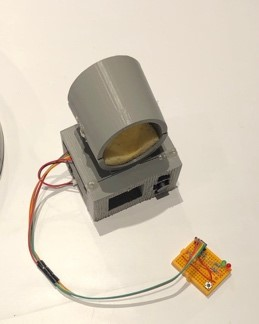
\includegraphics{hovertopview}
\caption{A top view of the Hover device. A wired controller with LED indicators can be seen.  The front panel with the sensors can also be seen.}
\end{figure}

\begin{figure}
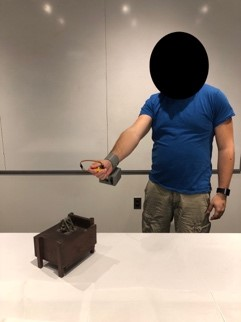
\includegraphics{hoverinteraction}
\caption{A user utilizing Hover to identify an object of interest.}
\end{figure}
\section{Evaluation}

We evaluated the user interactions of the system to see if it is a feasible alternative to head mounted devices and cellphones and the system's actual classification performance to see how the sensor fusion compares to a single sensor (camera) approach.  With regards to the user interaction aspect of the project, we developed an identification task in which we placed participants in a predetermined environment to identify a set of objects with a certain device (Hover, Hololens, and an Android Phone as the control). By doing this, we evaluated how users would feel about the devices in the general task of identifying some objects and getting information related to the objects. This task was meant to simulate an information gathering situation such as when a user is in a museum, or when a user would be shopping and trying to find additional information on an item of interest.  We asked the following set of questions and collected answers in a 5-point Likert scale:  

\begin{itemize}
    \item I think that I would like to use this system frequently. 
    \item I found the system unnecessarily complex.
    \item I thought the system was easy to use.
    \item I think that I would need the support of a technical person to be able to use this system.
    \item I found the various functions in this system were well integrated.	
    \item I thought there was too much inconsistency in this system.
    \item I would imagine that most people would learn to use this system very quickly.
    \item I found the system very cumbersome to use.
    \item I felt very confident using the system.	
    \item I needed to learn a lot of things before I could get going with this system.	
    \item What did you like about this system?	
    \item What did you dislike about this system?	
    \item How would you improve this system?
    \item How did this system compare to the others you used today?	
\end{itemize}
 

After analyzing the results, we found that Hover is comparable in cumbersomeness with a mobile phone, and less cumbersome than the head worn Hololens. Also, that Hover is not more immersive than a Hololens, but it is comparable in lack of immersiveness with a phone and a Hololens. We can also say that Hover is comparably less interruptive than a phone, and that it is comparable in interruptiveness with all the other devices in the study. We can also say that it is comparably less intrusive with a mobile phone, but that it is less intrusive than the head-worn Hololens. With regards to the multi-modal sensing, we found that the Hover system is slightly better than a plain camera without any sort of optimization, and the performance could possibly be improved if we replaced the radar module with one that has more bandwidth and range resolution, and we install a broadband Infra-Red (IR) led for our Near IR Spectrometer. Additionally, performance of the system could be further improved if parameter optimization were done either on the SVM classifier or on the K-Nearest neighbors classifier. 




\section{Conclusions}
In this work we proposed, designed, and implemented (at least in a proof of concept
way) a wearable object identification system that uses multi-modal sensing to be
able to identify objects. We began by first posing the idea of an alternate way of
124
accessing augmented reality content through wearables, and proceeded to come up
with a wrist-worn concept which we then implemented. Although the resulting form
factor was not optimal, we believe that it can be streamlined more with smaller, and
unied components.
After a user study on an object identification task, we can say the following. The hover
device is comparable in cumbersomeness with a mobile phone, and less cumbersome
than the head worn Hololens. It is not more immersive than a Hololens, but that it
is comparable in lack of immersiveness with a phone and a Hololens. We can also
say that it is comparably less interruptive than a phone, and that it is comparable
in interruptiveness with all the other devices in the study. We can also say that it is
comparably less intrusive with a mobile phone, but that it is less intrusive than the
head-worn Hololens.
With regards to the multi-modal sensing, we can see that it is slightly better than
a plain camera without any sort of optimization, and the performance could be improved
if we replaced the radar module with one that has more bandwidth and range
resolution, and we replaced the LED on the IR spectrometer. The LED that the spectrometer
currently has operates on one wavelength. To get better readings, we would
need to find a broadband IR led that we could use to see how objects respond and different
wavelengths. Performance could be further improved if parameter optimization
were done either on the SVM classifier or on the K-Nearest neighbors classifier.

\section{Future Work}
For future work we have a couple of areas that can be improved. The most prevalent
is the form factor. The form factor could be improved if we could streamline the
electronics into one board and somehow redistribute the antennas in a wider, but less
tall arrangement. Also, if we could find a smaller integrated board that would also
125
serve to shrink the overall footprint. The ideal form factor would be less than an inch
thick on the bottom of the device rather than the 3 inches that we currently have.
This would improve the overall experience as the device would blend in more with a
person rather than being an alien object on the body due to the size.
Additionally, we would attach a laser pointer to the device to give the users an idea
of where they are pointing the device to. We also note that there is a bug in the Bluetooth system of the NanoPi which produces choppy audio if it is not constant.
Other future work is finding more features for the sensing modalities and possibly
replacing the classification system with a pre-trained neural network, with a possible
convolutional component for the radar data. Other future work that can be done
is the automation of the hovering gesture rather than utilizing a button. The last
component that could be improved in future iterations is the Intelligent Assistant. If it
could be made more dynamic, both in its retrieval and presentation of the information,
then the system would be much more interactive.
%\end{document}  % This is where a 'short' article might terminate



% \appendix
% %Appendix A
% \section{Headings in Appendices}
% The rules about hierarchical headings discussed above for
% the body of the article are different in the appendices.
% In the \textbf{appendix} environment, the command
% \textbf{section} is used to
% indicate the start of each Appendix, with alphabetic order
% designation (i.e., the first is A, the second B, etc.) and
% a title (if you include one).  So, if you need
% hierarchical structure
% \textit{within} an Appendix, start with \textbf{subsection} as the
% highest level. Here is an outline of the body of this
% document in Appendix-appropriate form:
% \subsection{Introduction}
% \subsection{The Body of the Paper}
% \subsubsection{Type Changes and  Special Characters}
% \subsubsection{Math Equations}
% \paragraph{Inline (In-text) Equations}
% \paragraph{Display Equations}
% \subsubsection{Citations}
% \subsubsection{Tables}
% \subsubsection{Figures}
% \subsubsection{Theorem-like Constructs}
% \subsubsection*{A Caveat for the \TeX\ Expert}
% \subsection{Conclusions}
% \subsection{References}
% Generated by bibtex from your \texttt{.bib} file.  Run latex,
% then bibtex, then latex twice (to resolve references)
% to create the \texttt{.bbl} file.  Insert that \texttt{.bbl}
% file into the \texttt{.tex} source file and comment out
% the command \texttt{{\char'134}thebibliography}.
% % This next section command marks the start of
% % Appendix B, and does not continue the present hierarchy
% \section{More Help for the Hardy}

% Of course, reading the source code is always useful.  The file
% \path{acmart.pdf} contains both the user guide and the commented
% code.

\begin{acks}

This research has been supported by consortium funding at the MIT Media Laboratory. 

\end{acks}

% \subsection{Type Changes and {\itshape Special} Characters}

% We have already seen several typeface changes in this sample.  You can
% indicate italicized words or phrases in your text with the command
% \texttt{{\char'134}textit}; emboldening with the command
% \texttt{{\char'134}textbf} and typewriter-style (for instance, for
% computer code) with \texttt{{\char'134}texttt}.  But remember, you do
% not have to indicate typestyle changes when such changes are part of
% the \textit{structural} elements of your article; for instance, the
% heading of this subsection will be in a sans serif\footnote{Another
%   footnote here.  Let's make this a rather long one to see how it
%   looks.} typeface, but that is handled by the document class file.
% Take care with the use of\footnote{Another footnote.}  the
% curly braces in typeface changes; they mark the beginning and end of
% the text that is to be in the different typeface.

% You can use whatever symbols, accented characters, or non-English
% characters you need anywhere in your document; you can find a complete
% list of what is available in the \textit{\LaTeX\ User's Guide}
% \cite{Lamport:LaTeX}.

% \subsection{Math Equations}
% You may want to display math equations in three distinct styles:
% inline, numbered or non-numbered display.  Each of
% the three are discussed in the next sections.

% \subsubsection{Inline (In-text) Equations}
% A formula that appears in the running text is called an
% inline or in-text formula.  It is produced by the
% \textbf{math} environment, which can be
% invoked with the usual \texttt{{\char'134}begin\,\ldots{\char'134}end}
% construction or with the short form \texttt{\$\,\ldots\$}. You
% can use any of the symbols and structures,
% from $\alpha$ to $\omega$, available in
% \LaTeX~\cite{Lamport:LaTeX}; this section will simply show a
% few examples of in-text equations in context. Notice how
% this equation:
% \begin{math}
%   \lim_{n\rightarrow \infty}x=0
% \end{math},
% set here in in-line math style, looks slightly different when
% set in display style.  (See next section).

% \subsubsection{Display Equations}
% A numbered display equation---one set off by vertical space from the
% text and centered horizontally---is produced by the \textbf{equation}
% environment. An unnumbered display equation is produced by the
% \textbf{displaymath} environment.

% Again, in either environment, you can use any of the symbols
% and structures available in \LaTeX\@; this section will just
% give a couple of examples of display equations in context.
% First, consider the equation, shown as an inline equation above:
% \begin{equation}
%   \lim_{n\rightarrow \infty}x=0
% \end{equation}
% Notice how it is formatted somewhat differently in
% the \textbf{displaymath}
% environment.  Now, we'll enter an unnumbered equation:
% \begin{displaymath}
%   \sum_{i=0}^{\infty} x + 1
% \end{displaymath}
% and follow it with another numbered equation:
% \begin{equation}
%   \sum_{i=0}^{\infty}x_i=\int_{0}^{\pi+2} f
% \end{equation}
% just to demonstrate \LaTeX's able handling of numbering.

% \subsection{Citations}
% Citations to articles~\cite{bowman:reasoning,
% clark:pct, braams:babel, herlihy:methodology},
% conference proceedings~\cite{clark:pct} or maybe
% books \cite{Lamport:LaTeX, salas:calculus} listed
% in the Bibliography section of your
% article will occur throughout the text of your article.
% You should use BibTeX to automatically produce this bibliography;
% you simply need to insert one of several citation commands with
% a key of the item cited in the proper location in
% the \texttt{.tex} file~\cite{Lamport:LaTeX}.
% The key is a short reference you invent to uniquely
% identify each work; in this sample document, the key is
% the first author's surname and a
% word from the title.  This identifying key is included
% with each item in the \texttt{.bib} file for your article.

% The details of the construction of the \texttt{.bib} file
% are beyond the scope of this sample document, but more
% information can be found in the \textit{Author's Guide},
% and exhaustive details in the \textit{\LaTeX\ User's
% Guide} by Lamport~\shortcite{Lamport:LaTeX}.

% This article shows only the plainest form
% of the citation command, using \texttt{{\char'134}cite}.

% Some examples.  A paginated journal article \cite{Abril07}, an enumerated
% journal article \cite{Cohen07}, a reference to an entire issue \cite{JCohen96},
% a monograph (whole book) \cite{Kosiur01}, a monograph/whole book in a series (see 2a in spec. document)
% \cite{Harel79}, a divisible-book such as an anthology or compilation \cite{Editor00}
% followed by the same example, however we only output the series if the volume number is given
% \cite{Editor00a} (so Editor00a's series should NOT be present since it has no vol. no.),
% a chapter in a divisible book \cite{Spector90}, a chapter in a divisible book
% in a series \cite{Douglass98}, a multi-volume work as book \cite{Knuth97},
% an article in a proceedings (of a conference, symposium, workshop for example)
% (paginated proceedings article) \cite{Andler79}, a proceedings article
% with all possible elements \cite{Smith10}, an example of an enumerated
% proceedings article \cite{VanGundy07},
% an informally published work \cite{Harel78}, a doctoral dissertation \cite{Clarkson85},
% a master's thesis: \cite{anisi03}, an online document / world wide web
% resource \cite{Thornburg01, Ablamowicz07, Poker06}, a video game (Case 1) \cite{Obama08} and (Case 2) \cite{Novak03}
% and \cite{Lee05} and (Case 3) a patent \cite{JoeScientist001},
% work accepted for publication \cite{rous08}, 'YYYYb'-test for prolific author
% \cite{SaeediMEJ10} and \cite{SaeediJETC10}. Other cites might contain
% 'duplicate' DOI and URLs (some SIAM articles) \cite{Kirschmer:2010:AEI:1958016.1958018}.
% Boris / Barbara Beeton: multi-volume works as books
% \cite{MR781536} and \cite{MR781537}.

% A couple of citations with DOIs: \cite{2004:ITE:1009386.1010128,
%   Kirschmer:2010:AEI:1958016.1958018}.

% Online citations: \cite{TUGInstmem, Thornburg01, CTANacmart}.


% \subsection{Tables}
% Because tables cannot be split across pages, the best
% placement for them is typically the top of the page
% nearest their initial cite.  To
% ensure this proper ``floating'' placement of tables, use the
% environment \textbf{table} to enclose the table's contents and
% the table caption.  The contents of the table itself must go
% in the \textbf{tabular} environment, to
% be aligned properly in rows and columns, with the desired
% horizontal and vertical rules.  Again, detailed instructions
% on \textbf{tabular} material
% are found in the \textit{\LaTeX\ User's Guide}.

% Immediately following this sentence is the point at which
% Table~\ref{tab:freq} is included in the input file; compare the
% placement of the table here with the table in the printed
% output of this document.

% \begin{table}
%   \caption{Frequency of Special Characters}
%   \label{tab:freq}
%   \begin{tabular}{ccl}
%     \toprule
%     Non-English or Math&Frequency&Comments\\
%     \midrule
%     \O & 1 in 1,000& For Swedish names\\
%     $\pi$ & 1 in 5& Common in math\\
%     \$ & 4 in 5 & Used in business\\
%     $\Psi^2_1$ & 1 in 40,000& Unexplained usage\\
%   \bottomrule
% \end{tabular}
% \end{table}

% To set a wider table, which takes up the whole width of the page's
% live area, use the environment \textbf{table*} to enclose the table's
% contents and the table caption.  As with a single-column table, this
% wide table will ``float'' to a location deemed more desirable.
% Immediately following this sentence is the point at which
% Table~\ref{tab:commands} is included in the input file; again, it is
% instructive to compare the placement of the table here with the table
% in the printed output of this document.


% \begin{table*}
%   \caption{Some Typical Commands}
%   \label{tab:commands}
%   \begin{tabular}{ccl}
%     \toprule
%     Command &A Number & Comments\\
%     \midrule
%     \texttt{{\char'134}author} & 100& Author \\
%     \texttt{{\char'134}table}& 300 & For tables\\
%     \texttt{{\char'134}table*}& 400& For wider tables\\
%     \bottomrule
%   \end{tabular}
% \end{table*}
% % end the environment with {table*}, NOTE not {table}!

% It is strongly recommended to use the package booktabs~\cite{Fear05}
% and follow its main principles of typography with respect to tables:
% \begin{enumerate}
% \item Never, ever use vertical rules.
% \item Never use double rules.
% \end{enumerate}
% It is also a good idea not to overuse horizontal rules.


% \subsection{Figures}

% Like tables, figures cannot be split across pages; the best placement
% for them is typically the top or the bottom of the page nearest their
% initial cite.  To ensure this proper ``floating'' placement of
% figures, use the environment \textbf{figure} to enclose the figure and
% its caption.

% This sample document contains examples of \texttt{.eps} files to be
% displayable with \LaTeX.  If you work with pdf\LaTeX, use files in the
% \texttt{.pdf} format.  Note that most modern \TeX\ systems will convert
% \texttt{.eps} to \texttt{.pdf} for you on the fly.  More details on
% each of these are found in the \textit{Author's Guide}.

% \begin{figure}
% 
\includegraphics{fly}
% \caption{A sample black and white graphic.}
% \end{figure}





% As was the case with tables, you may want a figure that spans two
% columns.  To do this, and still to ensure proper ``floating''
% placement of tables, use the environment \textbf{figure*} to enclose
% the figure and its caption.  And don't forget to end the environment
% with \textbf{figure*}, not \textbf{figure}!

% \begin{figure*}
% 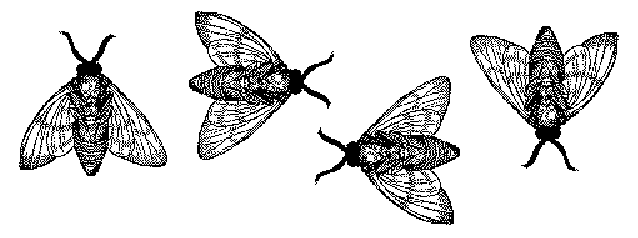
\includegraphics{flies}
% \caption{A sample black and white graphic
% that needs to span two columns of text.}
% \end{figure*}


% \begin{figure}
% 
\includegraphics[height=1in, width=1in]{rosette}
% \caption{A sample black and white graphic that has
% been resized with the \texttt{includegraphics} command.}
% \end{figure}

% \subsection{Theorem-like Constructs}

% Other common constructs that may occur in your article are the forms
% for logical constructs like theorems, axioms, corollaries and proofs.
% ACM uses two types of these constructs:  theorem-like and
% definition-like.

% Here is a theorem:
% \begin{theorem}
%   Let $f$ be continuous on $[a,b]$.  If $G$ is
%   an antiderivative for $f$ on $[a,b]$, then
%   \begin{displaymath}
%     \int^b_af(t)\,dt = G(b) - G(a).
%   \end{displaymath}
% \end{theorem}

% Here is a definition:
% \begin{definition}
%   If $z$ is irrational, then by $e^z$ we mean the
%   unique number that has
%   logarithm $z$:
%   \begin{displaymath}
%     \log e^z = z.
%   \end{displaymath}
% \end{definition}

% The pre-defined theorem-like constructs are \textbf{theorem},
% \textbf{conjecture}, \textbf{proposition}, \textbf{lemma} and
% \textbf{corollary}.  The pre-defined de\-fi\-ni\-ti\-on-like constructs are
% \textbf{example} and \textbf{definition}.  You can add your own
% constructs using the \textsl{amsthm} interface~\cite{Amsthm15}.  The
% styles used in the \verb|\theoremstyle| command are \textbf{acmplain}
% and \textbf{acmdefinition}.

% Another construct is \textbf{proof}, for example,

% \begin{proof}
%   Suppose on the contrary there exists a real number $L$ such that
%   \begin{displaymath}
%     \lim_{x\rightarrow\infty} \frac{f(x)}{g(x)} = L.
%   \end{displaymath}
%   Then
%   \begin{displaymath}
%     l=\lim_{x\rightarrow c} f(x)
%     = \lim_{x\rightarrow c}
%     \left[ g{x} \cdot \frac{f(x)}{g(x)} \right ]
%     = \lim_{x\rightarrow c} g(x) \cdot \lim_{x\rightarrow c}
%     \frac{f(x)}{g(x)} = 0\cdot L = 0,
%   \end{displaymath}
%   which contradicts our assumption that $l\neq 0$.
% \end{proof}

\bibliographystyle{ACM-Reference-Format}
\bibliography{sample-bibliography}

\end{document}
